\section{Clustering}
\textcolor{blue}{k} Anzahl Clusters die es geben darf (Hyperparameter)

\subsection{Unsupervised Learning}
\begin{itemize}
    \item We are given Data (features, x) wihout labels (y)
    \item It learns something through the structure of the data
\end{itemize}
\vspace{10pt}
\textbf{The goal}

self-discover patterns from the data \\

\textbf{Clusters}
\begin{itemize}
    \item Data points which have shared properties
    \item Fall into one cluster or one alike group
    \item Similar Data Points are close together
    \item \textcolor{blue}{Group $n$ data points into $k_c$ number of clusters}
\end{itemize}
\vspace{10pt}
\textbf{Applications}
\begin{itemize}
    \item Social Network Analysis
    \item Astronomical Data
    \item Marked segmentation
    \item Recommendation systems
\end{itemize}
\subsection{Naive K-means}
%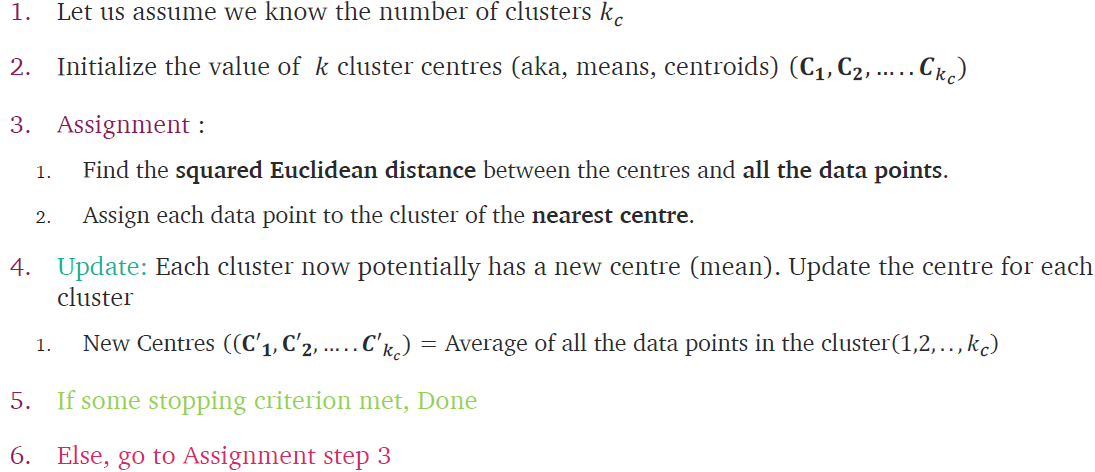
\includegraphics[width=\linewidth]{k-means.png}

\begin{enumerate}
    \item Gehen wir davon aus wir kennen die Anzahl Clusters $k$
    \item Initialisiere $k$ Cluster Centers (aka means, centroids)
    \item Assignment
        \begin{enumerate}
            \item Finde die \textcolor{blue}{squared Euclidean Distance} \\ $d_{ik} = (x_i - C_k)^2$ \\ zwischen Center und \textcolor{blue}{allen Datenpunkten}
            \item Weise jeden Datenpunkt dem \textcolor{blue}{nächsten} Center zu
        \end{enumerate}
    \item Update: Jedes Cluster hat nun möglicherweise ein neues Center. Update des Center aller Clusters \\ $C_k = \frac{1}{size(C_k)} \sum_{x_i \in cluster k} x_i$
    \item Wenn Stopping Kriterium, Fertig
    \item Sonst gehen zu Assignment
\end{enumerate}
\vspace{10pt}
%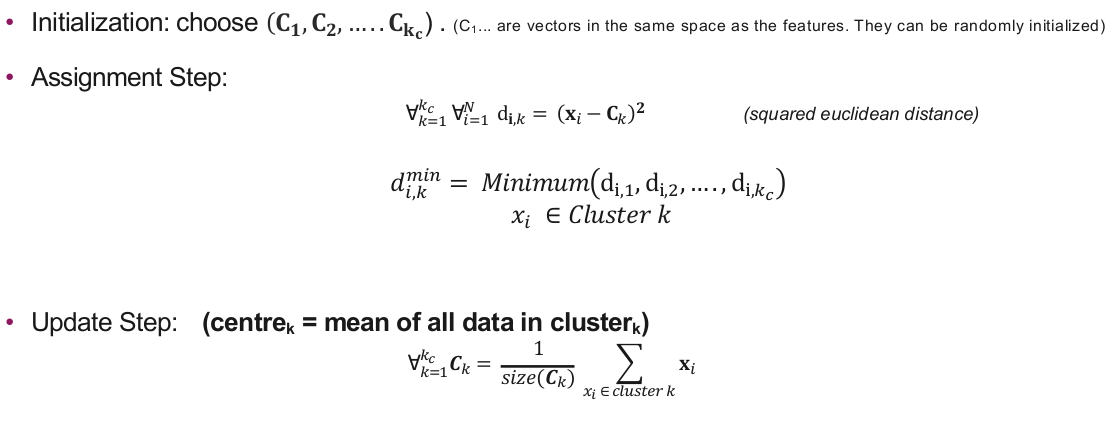
\includegraphics[width=\linewidth]{clusters-formal-maths.png} \\

\textbf{Example}

\textcolor{blue}{Calculating cluster centre}

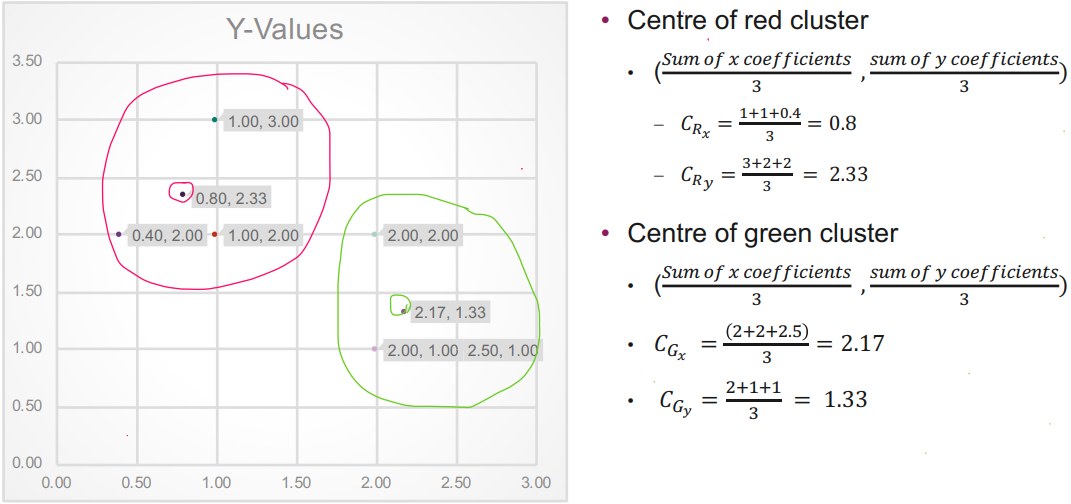
\includegraphics[width=\linewidth]{k-means-example-1.png} \\

\textcolor{blue}{Assignment of a point to cluster}

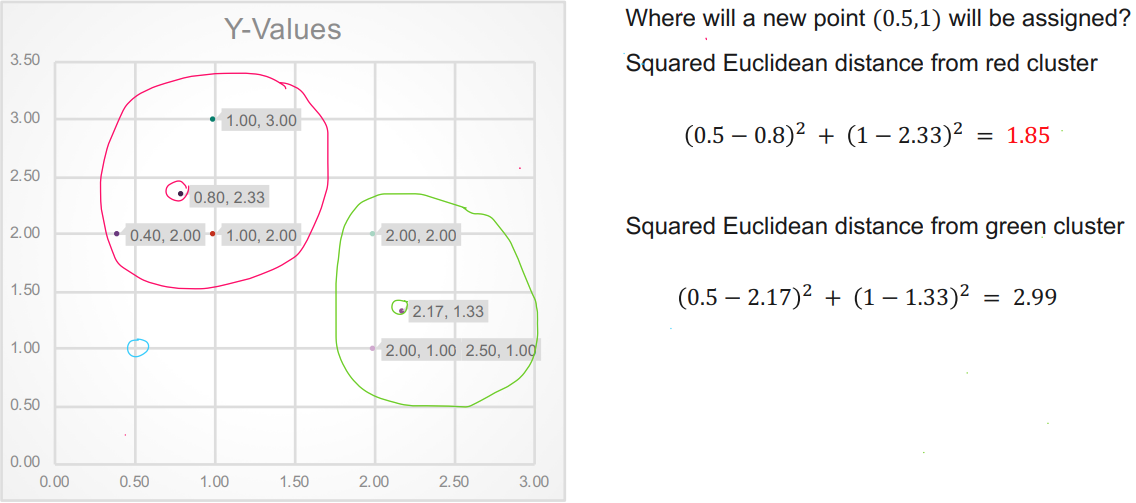
\includegraphics[width=\linewidth]{k-means-example-2.png} \\

New point will assigned to the red cluster. The center of this cluster must be recalculated

$C_R = (\frac{1+1+.4+0.5}{4} , \frac{3+2+2+1}{4}) = (0.97, 2.7)$ \\

\begin{minipage}[t]{0.5\linewidth}
    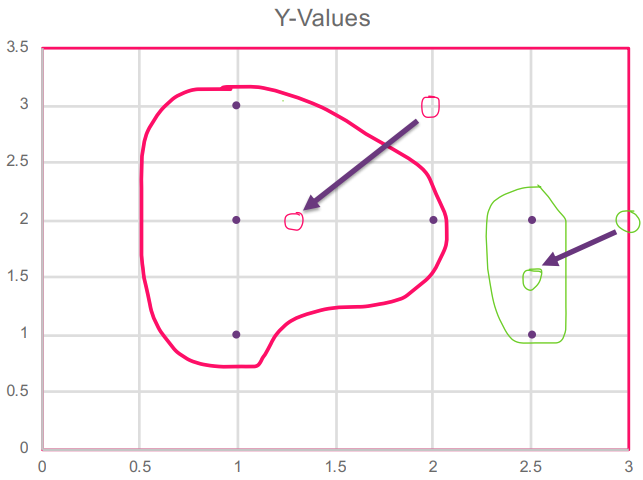
\includegraphics[width=\linewidth]{k-means-example-3.png}
\end{minipage}
\begin{minipage}[t]{0.5\linewidth}
    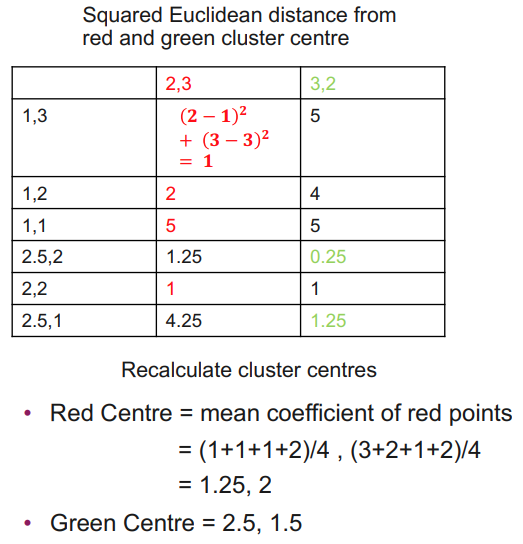
\includegraphics[width=\linewidth]{k-means-example-4.png}
\end{minipage}


\subsubsection{Stopping Criterion}
\begin{itemize}
    \item When centers don't change (time consuming)
    \item The datapoints assigned to specific cluster remains the same (takes too much time)
    \item The distance of datapoints from their centres $>=$ treshold we have set
    \item Fixed number of iterations have reached
\end{itemize}

\subsubsection{Initialization}
\begin{itemize}
    \item Performance depends on the random initialization
    \item Some seeds can result in a poor convergence rate
    \item Some seeds can converge to suboptimal clustering
    \item If centres are very close, it takes a lot of iterations to converge
    \item Initialize randomly, run multiple times
\end{itemize}

\subsubsection{Standardization of data}
\begin{itemize}
    \item Features with large values may dominate the distance value
    \item Features over small values will have no impact
    \item Normalize values, apply scaling!
\end{itemize}

\subsection{Sklean k-means}
\textbf{Initialization}
\begin{itemize}
    \item Init = K-means$++$
    \item Only initialization of the centroids will change
    \item Chosen centroids should be far from each other
\end{itemize}
\vspace{10pt}
\textcolor{blue}{max\_iter} Number of iterations before stopping \\

\textcolor{blue}{n\_init} Number of time the k-means algorithm will be run with different centroid seeds

\vfill\null
\columnbreak
\subsection{Evaluate Cluster Quality}
Make clusters so that for each cluster the distance of each cluster member from its center is minimizes \\

\textbf{Inertia or within-cluster sum-of-squares (WCSS)}
\begin{itemize}
    \item Sum of squared distances of samples (each point) to their closest center
    \item As small as possible
    \item \textcolor{blue}{Dort wo der Knick ist, ist am besten ''Elbow''}
\end{itemize}

\begin{minipage}[t]{0.5\linewidth}
    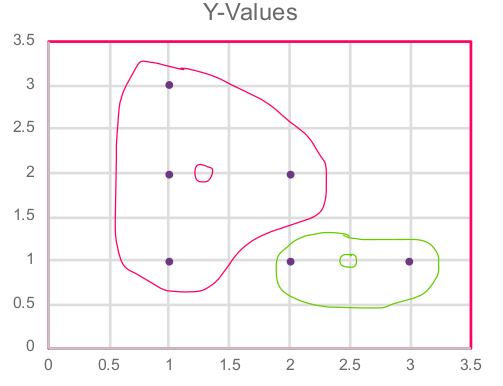
\includegraphics[width=\linewidth]{wcss-diagram.png}
\end{minipage}
\begin{minipage}[t]{0.5\linewidth}
    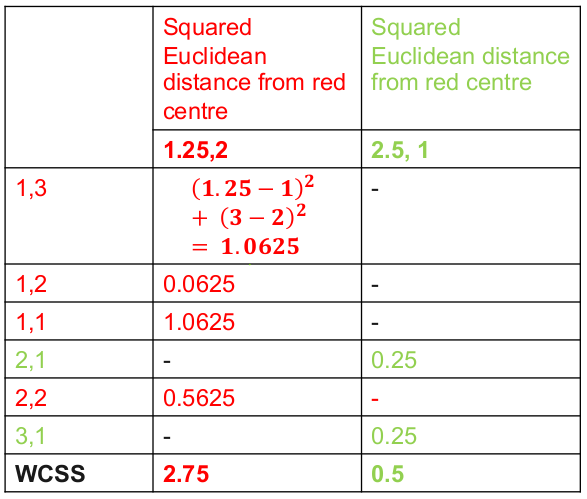
\includegraphics[width=\linewidth]{wcss-table.png}
\end{minipage}
\vspace{10pt}
\textbf{Silhouette Score}
\begin{itemize}
    \item How far the datapoints in one cluster are from the datapoints in another cluster
    \item \textcolor{blue}{Silhouette Score of a point} $\frac{b-a}{max(a,b)}$
    \begin{itemize}
        \item \textcolor{blue}{a} average intra-cluster distance (distance between each point within)
        \item \textcolor{blue}{b} average inter-cluster distance (distance between a cluster and its nearest neighbour)
    \end{itemize}
\end{itemize}
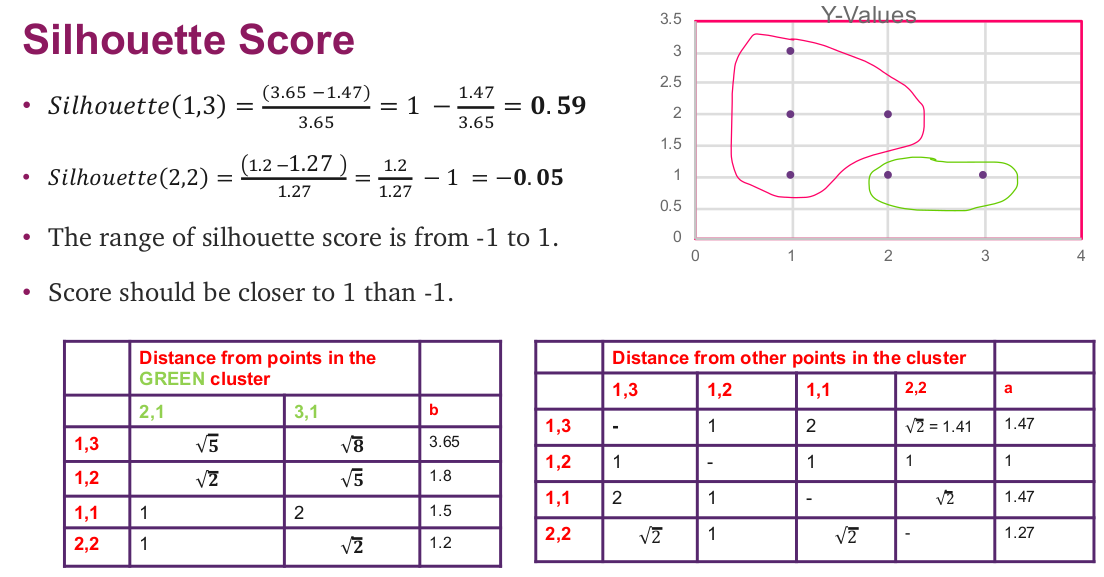
\includegraphics[width=0.8\linewidth]{silhouette-score.png}

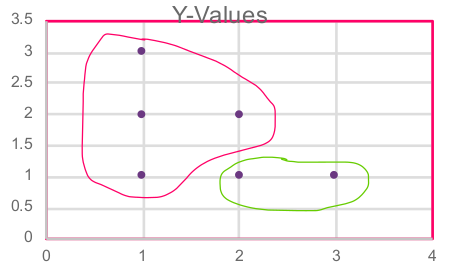
\includegraphics[width=0.6\linewidth]{silhouette-score-1.png}

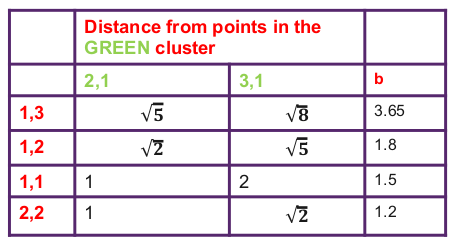
\includegraphics[width=0.8\linewidth]{silhouette-score-2.png}

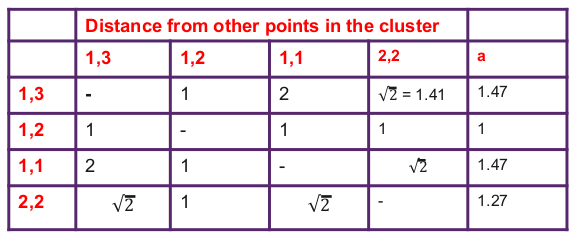
\includegraphics[width=0.8\linewidth]{silhouette-score-3.png}

